% !TeX spellcheck = it_IT
% !TeX root = ../it.tex

\chapter{Teoria della Complessità}

Dato un problema $P$, fino a ora la domanda è stata "\textit{esiste un programma per la sua soluzione automatica?}" E tramite questa domanda si può indagare la teoria della calcolabilità, il cui soggetto di studio è l'esistenza (o meno) di un programma per un dato problema.

La prossima sezione riguarda la \textbf{teoria della complessità} in cui l'investigazione segue la domanda "\textit{come funzionano i programmi per $P$?}".

Per rispondere a questa domanda, vogliamo sapere quante \textbf{risorse computazionali} vengono utilizzate durante la sua esecuzione. Vediamo altre domande a cui la teoria della complessità cerca di rispondere
\begin{itemize}
	\item dato un programma per il problema $P$, quanto tempo impiega nella sua soluzione? Quanto spazio di memoria occupa? 
	\item dato un problema $P$, qual è il minimo tempo impiegato dai programmi per $P$? Quanto spazio in memoria al minimo posso occupare per programmi per $P$? 
	\item in che senso possiamo dire che un programma è \textbf{efficiente} in termini di tempo e/o spazio? 
	\item quali problemi possono essere efficientemente risolti per via automatica?
\end{itemize}

\section{Teoria dei linguaggi formali}

Alcune definizioni:
\begin{itemize}
	\item Un \textbf{alfabeto} è un insieme finito di simboli $\Sigma = \{\sigma_1, \dots, \sigma_k\}$
	\item Un \textbf{alfabeto binario} è un qualsiasi alfabeto composto da due soli simboli
	\item Una \textbf{stringa} su $\Sigma$ è una sequenza di simboli appartenenti a $\Sigma$ nella forma $x = x_1 \cdots x_n$, con $x_i \in \Sigma$
	\item La \textbf{lunghezza} di una stringa $x$ indica il numero di simboli che la costituiscono e si indica con $|x|$
	\item La \textbf{stringa nulla} è una stringa particolare, indicata con $\epsilon$, è tale che $|\epsilon| = 0$
	\item Con $\Sigma^\ast$ si indica l'insieme delle stringhe che si possono costruire sull'alfabeto $\Sigma$ (chiusura di Kleene), compresa la stringa nulla. L'insieme delle stringhe formate da almeno un carattere è $\Sigma^+ = \Sigma^\ast \setminus \{\epsilon\}$
	\item Un \textbf{linguaggio} $L$ su un alfabeto $\Sigma$ è un sottoinsieme $L \subseteq \Sigma^\ast$, che può essere finito o infinito
\end{itemize}

\section{Macchina di Turing Deterministica (DTM)}
Il punto di partenza dello studio della teoria della complessità e la definizione rigorosa delle risorse di calcolo e di come possono essere misurate.

Il modello di calcolo considerato è quello della \textbf{Macchina di Turing}, ideata da Alan Turing nel 1936. Si tratta di un modello teorico di calcolatore che consente di definire rigorosamente: 
\begin{itemize}
	\item i passi di computazione e la computazione stessa
	\item tempo e spazio di calcolo dei programmi
\end{itemize}

\subsection{Struttura}
Una \textbf{Macchina di Turing deterministica} è un dispositivo hardware fornito di: 
\begin{itemize}
	\item \textbf{nastro di lettura/scrittura}: un nastro infinito formato da celle, ognuna delle quali ha un proprio indice/indirizzo e può contenere un simbolo. Questo nastro viene usato come contenitore per l'input, ma anche come memoria durante l'esecuzione
	\item \textbf{testina di lettura e scrittura two-way}: dispositivo che permette di leggere e scrivere dei simboli sul nastro a ogni passo
	\item \textbf{controllo a stati finiti}: automa a stati finiti $Q = \{Q_0, \dots, Q_n\}$ che permette di far evolvere la computazione
\end{itemize}

Un passo di calcolo è una \textbf{mossa} che, dato lo stato corrente e il simbolo letto dalla testina, porta la DTM in un nuovo stato, scrivendo eventualmente un simbolo sul nastro e spostando eventualmente la testine. I risultati della mossa, quindi il nuovo stato, il simbolo da scrivere e il movimento della testina, vengono calcolati tramite una \textbf{funzione di transizione}, basata sui due input dati.

\subsubsection{Definizione Informale}

Il funzionamento di una DTM $M$ su input $x \in \Sigma^\ast$ passa per due fasi:
\begin{enumerate}
	\item \textbf{Inizializzazione}:
	\begin{itemize}
		\item La stringa $x$ viene posta, simbolo dopo simbolo, nelle celle del nastro dalla cella 1 fino alla cella $|x|$. Le celle dopo quelle che contengono $x$ contengono il simbolo \textit{blank}
		\item La testina si posizione sulla prima cella
		\item Il controllo a stati finiti è posto nello stato iniziale
	\end{itemize}
	\item \textbf{Computazione}:
	\begin{itemize}
		\item Sequenza di mosse dettata dalla funzione di transizione
	\end{itemize}
\end{enumerate}

La computazione può andare in loop o arrestarsi se raggiunge una situazione in cui non è definita nessuna mossa per lo stato attuale. Si dice che $M$ accetta $x \in \Sigma^\ast$ se $M$ si arresta in uno stato tra quelli finali/accettanti, altrimenti la rifiuta.

Definiamo $L_M = \{x \in \Sigma^\ast \mid M \text{ accetta } x \}$ il \textbf{linguaggio accettato} da $M$.

\subsubsection{Definizione Formale}
Una DTM è una sestupla $M = \left(Q, \Sigma, \Gamma, \delta, q_0, F\right)$, con:
\begin{itemize}
	\item $Q$: insieme finito di \textbf{stati} assumibili dal controllo a stati finiti
	\item $q_0 \in Q$: \textbf{stato iniziale} da cui partono le computazioni di $M$
	\item $F \subseteq Q$: insieme degli \textbf{stati finali/accettanti} dove $M$ si arresta accettando l'input
	\item $\Sigma$: \textbf{alfabeto di input} su cui sono definite le stringhe di input
	\item $\Gamma$: \textbf{alfabeto di lavoro} che contiene i simboli che possono essere letti/scritti dal/sul nastro. Vale $\Sigma \subset \Gamma$ perché $\Gamma$ contiene il simbolo \textit{blank}
	\item $\delta: Q \times \Gamma \rightarrow Q \times (\Gamma \setminus \{blank\}) \times \{-1, 0, 1\}$: \textbf{funzione di transizione} che definisce le mosse. Si tratta di una funzione parziale: quando non è definita la macchina si arresta. Inoltre, $M$ non può scrivere il simbolo \textit{blank}, lo può solo leggere
\end{itemize}

Analizziamo nel dettaglio lo sviluppo di una DTM $M$ su input $x \in \Gamma^\ast$, visto solo informalmente: 
\begin{enumerate}
	\item \textbf{Inizializzazione}: 
	\begin{itemize}
		\item il nastro contiene la stringa $x = x_1 \cdots x_n$
		\item la testina è posizionata sul carattere $x_1$
		\item il controllo a stati finiti parte dallo stato $q_0$
	\end{itemize}
	\item \textbf{Computazione}: sequenza di mosse definite dalla funzione di transizione $\delta$ che manda, a ogni passo, da $(q_i, \gamma_i)$ a $(q_{i+1}, \gamma_{i+1}, \{-1, 0, +1\})$
\end{enumerate}

Se $\delta(q, \gamma) = \bot$, la macchina $M$ si \textit{arresta}. Quando la testina rimbalza tra due celle o rimane fissa in una sola, si verifica un \textit{loop}. La macchina $M$ accetta $x \in \Sigma^\ast$ se e solo se la computazione si arresta in uno stato $q \in F$. \lcomment{Guarda foto se vuoi Slide 18:9} Come prima, $L_M = \{x \in \Sigma^\ast \mid M \text{ accetta } x\}$ è il \textbf{linguaggio accettato} da $M$.

Queste macchine sono molto simili agli automi a stati finiti, seppur con alcune differenze: 
\begin{itemize}
	\item le FSM di default non possono tornare indietro, non sono two-way, ma questa differenza non aumenta la potenza computazionale, serve solo per avere automi più succinti
	\item le FSM hanno il nastro a sola lettura, mentre le DTM possono alterare il nastro a disposizione
\end{itemize}

\subsubsection{Configurazione di una DTM}

Proviamo, similmente a come fatto per le macchine $\ram$, a dare l'idea di \textbf{configurazione} delle DTM; possiamo vederla come una foto che descrive completamente la macchina $M$ in un certo istante, in questo modo possiamo descrivere la computazione come usa serie di configurazioni/foto.

Le cose da ricordare sono: 
\begin{itemize}
	\item in che stato si trova la macchina
	\item in che posizione si trova la testina
	\item il contenuto non-blank del nastro
\end{itemize}

Definiamo quindi $C = (q,k,w)$ una configurazione con
\begin{itemize}
	\item $q$: stato del controllo a stati finiti
	\item $k \in \N^+$: posizione della testina nel nastro
	\item $w \in \Gamma^+$: contenuto non-blank del nastro
\end{itemize}

All'inizio della computazione si ha la \textbf{configurazione iniziale} $C_0 = (q_0, 1, x)$. Una configurazione $C$ si dice \textbf{accettante} se $C = (q \in F, k, w)$, si dice invece \textbf{d'arresto} se $C = (q, k, w)$, con $\delta (q,w_{k}) = \bot$.

\subsubsection{Definizione di computazione tramite configurazioni}

La computazione di $M$ su $x \in \Sigma^\ast$ è la sequenza
$$ C_0 \xrightarrow{\delta} C_1 \xrightarrow{\delta} \dots \xrightarrow{\delta} C_i \xrightarrow{\delta} C_{i+1} \xrightarrow{\delta} \dots $$
dove $\forall i \geq 0$ vale che da $C_i$ si passa a $C_{i+1}$ grazie alla funzione $\delta$.

La macchina $M$ accetta $x \in \Sigma^\ast$ se e solo se $C_0 \xrightarrow{\ast}C_f$, con $C_f$ configurazione d'arresto e accettante. Il linguaggio accettato da $M$ ha la stessa definizione data prima.

\subsection{Altre versioni delle macchine di Turing}
\subsubsection{Versioni alternative}

Il fatto che la macchina sia \textit{deterministica} implica che, data una configurazione $C_i$, quella successiva è univocamente determinata dalla funzione $\delta$. Quindi, data una configurazione $C_i$, esiste una sola configurazione $C_{i+1}$ successiva, a meno di arresti. \lcomment{Guarda foto se vuoi 18:11}

Nelle \textbf{Macchine di Turing Non Deterministiche (NDTM)}, una configurazione $C_i$ può ammettere più configurazioni successive.

Nelle \textbf{Macchine di Turing Probabilistiche PTM}, data una configurazione $C_i$, possono esistere più configurazioni nelle quali si può entrare, ognuna associata a una probabilità $p_i \in [0,1]$.

Infine, nelle \textbf{Macchine di Turing Quantistiche QTM}, data una configurazione $C_i$, esistono una serie di configurazioni successive nelle quali possiamo entrare osservando le ampiezze delle transizioni $\alpha_i$. Queste ampiezze sono numeri complessi in $\mathbb{C}$ tali che
\begin{itemize}
	\item $|\alpha_i| \leq 1$
	\item hanno probabilità $|\alpha_i|^2$
	\item le probabilità sommano a 1
\end{itemize}

\subsubsection{Versione semplificata}
Esibire, progettare e comprendere una DTM potrebbe risultare difficile, anche per casi semplici. Solitamente, nel descrivere una DTM viene utilizzato uno \textit{pseudocodice} che ne chiarisce la dinamica.

Esistono una serie di teoremi che dimostrano che qualsiasi frammento di programma strutturato può essere tradotto in una DTM formale e viceversa.

\subsubsection{Esempio: parità}
Problema: 
\begin{itemize}
	\item Nome: parità
	\item Istanza: $x \in \N$
	\item Domanda: $x$ è pari?
\end{itemize}

Come codifica utilizziamo quella binaria, ovvero
$$ cod: \N \rightarrow \{0,1\}^\ast $$
Di conseguenza, il linguaggio da riconoscere è 
$$ L_{\text{pari}} = \left\{x \in \{0,1\}^\ast \mid x_1 = 1 \wedge x_{|x|} = 0 \right\} \cup \{0\} $$
Risolvere il problema \textit{parità} significa trovare una DTM $M$ che rappresenta un algoritmo deterministico che riconosce $L_{\text{pari}}$.

Ricordando che $M = \left(Q, \Sigma, \Gamma, \delta, q_0, F\right)$, la seguente macchina riconosce $L_{\text{pari}}$:
\begin{itemize}
	\item $Q = \{p, z_1, \mu, z, r\}$ insieme degli stati
	\item $\Sigma = \{0,1\}$ alfabeto 
	\item $\Gamma = \{0,1, blank\}$ alfabeto di lavoro
	\item $q_0 = p$ stato iniziale
	\item $F = \{z_1, z\}$ insieme degli stati finali
	\item $\delta : Q \times \Gamma \rightarrow Q \times \Sigma \times \{-1, 0, 1\}$ funzione di transizione così definita
	\begin{center}
		\renewcommand{\arraystretch}{1.5}
		\begin{tabular}{| C{40000cm} | C{40000cm} | C{40000cm} | C{40000cm} |}
			\hline
			$\delta$ & \textit{blank} & 0 & 1 \\
			\hline
			$p$ & $\bot$ & $(z_1, 0, +1)$ & $(\mu, 1, +1)$ \\
			\hline
			$z_1$ & $\bot$ & $(r, 0, +1)$ & $(\mu, 1, +1)$ \\
			\hline
			$\mu$ & $\bot$ & $(z, 0, +1)$ & $(\mu, 1, +1)$ \\
			\hline
			$z$ & $\bot$ & $(z, 0, +1)$ & $(\mu, 1, +1)$ \\
			\hline
			$r$ & $\bot$ & $\bot$ & $\bot$ \\
			\hline
		\end{tabular}
	\end{center}
\end{itemize}

Si può notare come, anche per un problema così semplice, si ha una funzione di transizione abbastanza complessa. Andiamo quindi a utilizzare uno pseudocodice:
\begin{center}
	\begin{minipage}{.7\textwidth}
		\begin{tcolorbox}[
			colback=white,
			sharp corners,
			boxrule=.3mm,
			left=20pt,
			top=0pt,
			bottom=0pt,
			title=Parità$(n)$,
			colbacktitle=white,
			coltitle=black
			]
			\LinesNumbered
			\begin{algorithm}[H]
				\setstretch{1.2}
				\SetArgSty{relax}
				\SetAlgoNoEnd
				\SetKwProg{if}{if}{}{}
				\SetKwProg{els}{else}{}{}
				\SetKwProg{Do}{do}{}{}
				\SetKwProg{While}{while}{}{}
				\SetKwSty{texttt}
				$i:=1$ \\
				$f:=false$ \\
				\Switch{$x[i]$}{
					\Case{0}{
						$i++$ \\
						$f:= (x[i] == blank)$ \\
						break\\
					}
					\Case{1}{
						\Do{}{
							$f:= (x[i] == 0)$ \\
							$i++$ \\
						}
						\While{$(x[i] \neq blank)$}{}
					}
				}
				\Return{$f$}
			\end{algorithm}
		\end{tcolorbox}
	\end{minipage}
\end{center}

Alla fine dell'esecuzione avremo: 
\begin{itemize}
	\item \textit{True} se $x \in L_{\text{pari}}$
	\item \textit{False} se $x \notin L_{\text{pari}}$
\end{itemize}

\section{Funzionalità di una DTM}

\subsection{Insiemi riconosciuti}

La principale funzionalità di una DTM è \textbf{riconoscere linguaggi}. Un linguaggio $L \subseteq \Sigma^\ast$ è \textbf{riconoscibile} da una DTM se e solo se esiste una DTM $M$ tale che $L = L_M$.

Grazie alla possibilità di riconoscere linguaggi, una DTM può riconoscere anche insiemi: dato $A \subseteq \N$, \textit{come lo riconosco con una DTM?} La prima idea è quella di codificare ogni elemento $a \in A$ in un elemento di $\Sigma^\ast$, per poter passare dal riconoscimento di un insieme al riconoscimento di un linguaggio.
$$
\renewcommand{\arraystretch}{1.8}
A \rightsquigarrow \begin{array}{|c|}
	\hline
	cod \\
	\hline
\end{array}
\rightsquigarrow L_A = \{cod(a): a \in A\}
$$

Un insieme $A$ è riconoscibile da una DTM se e solo se esiste una DTM $M$ tale che $L_A = L_M$.

Quando si fa riconoscere un insieme $A$ a una DTM $M$, possono risultare due situazioni, in funzione dell'input (codificato):
\begin{enumerate}
	\item se l'input appartiene ad $A$, allora $M$ si arresta
	\item se l'input \textit{non} appartiene ad $A$, allora $M$ può 
	\begin{itemize}
		\item arrestarsi rifiutando l'input, ovvero finisce in uno stato $q \notin F$, ma allora $A$ è ricorsivo
		\item andare in loop, ma allora $A$ è ricorsivamente numerabile \\
	\end{itemize}
\end{enumerate}

\begin{theor}
	La classe degli insiemi riconosciuti da una DTM coincide con la classe degli insiemi ricorsivamente numerabili.
\end{theor}

Un algoritmo deterministico per il riconoscimento di un insieme $A \subseteq \N$ è una DTM $M$ tale che $L_A = L_M$ e tale che $M$ si arresta su ogni input.\\

\begin{theor}
	La classe degli insiemi riconosciuti da algoritmi deterministici coincide con la classe degli insiemi ricorsivi.
  \end{theor}

% FINITO QUI DEVI FARE LEZIONE 19

\subsection{Problemi di decisione}

Una seconda funzionalità delle DTM è quella di risolvere \textbf{problemi di decisione}. Dato un problema $\Pi$, con istanza $x \in D$ e domanda $p(x)$, andiamo a codificare gli elementi di $D$ in elementi di $\Sigma^\ast$, ottenendo $L_\Pi = \{cod(x) \mid x \in D \wedge p(x) \}$ \textbf{insieme delle istanze (codificate) a risposta positiva di $\Pi$}.

La DTM risolve $\Pi$ se e solo se $M$ è un algoritmo deterministico per $L_\Pi$, ovvero: 
\begin{itemize}
	\item se vale $p(x)$, allora $M$ accetta la codifica di $x$
	\item se non vale $p(x)$, allora $M$ si arresta senza accettare
\end{itemize}

\subsection{Calcolo di funzioni}

Oltre a ciò che è già stato detto, le DTM sono anche in grado di \textbf{calcolare funzioni}. Si tratta di un risultato molto importante, in quanto sappiamo che calcolare funzioni significa risolvere problemi del tutto generali, quindi non solo di decisione.

Data una funzione $f: \Sigma^\ast \rightarrow \Gamma^\ast$, la DTM $M$ calcola $f$ se e solo se
\begin{itemize}
	\item se $f(x) \downarrow$ allora $M$ su input $x$ termina con $f(x)$ sul nastro
	\item se $f(x) \uparrow$ allora $M$ su input $x$ va in loop
\end{itemize}
A tutti gli effetti le DTM sono \textit{sistemi di programmazione}.

\subsection{Potenza computazionale}

Si può dimostrare che le DTM calcolano tutte e sole le funzioni ricorsive parziali. Possiamo riscrivere la tesi di Church-Turing come: 
\begin{center}
	\textit{Una funzione è intuitivamente calcolabile se e solo se è calcolata da una DTM}
\end{center}

Inoltre, è possibile dimostrare che le DTM sono SPA, semplicemente mostrando che valgono i tre assiomi di Rogers: 
\begin{enumerate}
	\item le DTM calcolano tutte e sole le funzioni ricorsive parziali 
	\item esiste una DTM universale che simula tutte le altre
	\item vale il teorema $S^m_n$
\end{enumerate}

\section{Simboli di Landau}

Nella teoria delle complessità la domanda è \textit{"quanto costa questo programma?"} Per capire il costo di un dato programma verranno valutate delle funzioni nella forma $f(n)$, dove $n$ indica la grandezza dell'input della DTM. Nel fare il confronto tra due algoritmi per uno stesso problema, bisogna tenere in considerazione che a fare la differenza (in termini di prestazioni) sono gli input di dimensione \textit{ragionevolmente grande}, dove con questa espressione intendiamo una dimensione significativa nel contesto d'applicazione del problema.

Per esempio, siano $t_1$ e $t_2$ due funzioni tali che
$$ t_1 (n) = 2n \quad \mid \quad t_2 (n) = \frac{1}{100} n^2 + \frac{1}{2}n + 1 $$

Quale delle due è migliore? \textit{Dipende}, per $n$ abbastanza piccoli allora $t_2$ è migliore, mentre per $n$ sufficientemente grandi allora è migliore $t_1$.

Date due funzioni, non vanno valutate per valori precisi di $n$, ma ne va valutato il loro \textbf{andamento asintotico}, ovvero quando $n$ tende a $+ \infty$.

\subsection{Simboli di Landau principali}

I \textbf{simboli di Landau} sono utili per stabilire degli \textbf{ordini di grandezza} tra le funzioni, in modo da poterle paragonare. I più utilizzati sono:
\begin{enumerate}
	\item $O$: date due funzioni $f,g: \N \rightarrow \N$ diciamo che 
	$$ f(n) = O(g(n)) $$
	se e solo se
	$$ \exists c > 0 \quad \exists n_0 \in \N \mid \forall n \geq n_0 \quad f(n) \leq c \cdot g (n) $$
	Fornisce un upper bound alla funzione $f$.
	
	\item $\Omega$: date due funzioni $f,g: \N \rightarrow \N$ diciamo che 
	$$ f(n) = \Omega (g(n)) $$
	se e solo se
	$$ \exists c > 0 \quad \exists n_0 \in \N \mid \forall n \geq n_0 \quad f(n) \geq c \cdot g (n) $$
	Fornisce un lower bound alla funzione $f$.
	
	\item $\Theta$: date due funzioni $f,g : \N \rightarrow \N$ diciamo che
	$$ f(n) = \Theta (g(n)) $$
	se e solo se
	$$ \exists c_1, c_2 > 0 \quad \exists n_0 \in \N \mid \forall n \geq n_0 \quad c_1 \cdot g(n) \leq f(n) \leq c_2 \cdot g(n) $$
\end{enumerate}

Si può notare facilmente che valgono le proprietà
$$ f(n) = O(g(n)) \Leftrightarrow g(n) = \Omega(f(n)) $$
$$ f(n) = \Theta(g(n)) \Leftrightarrow f(n) = O (g(n)) \wedge f(n) = \Omega(g(n)) $$

\section{Definizione della risorsa tempo}

Per \textit{semplicità} usiamo una DTM e non una macchina $\ram$ per dare una definizione rigorosa di tempo. Le $\ram$, per quanto semplici, lavorano con banchi di memoria che possono contenere dati di grandezza arbitraria ai quali si accede in tempo $O(1)$, cosa che invece non si può fare con le DTM perché il nastro contiene l'input diviso su più celle.

\subsection{Definizione}

Consideriamo la DTM $M = (Q, \Sigma, \Gamma, \delta, q_0, F)$ e definiamo
\begin{itemize}
	\item $T(x)$ il \textbf{tempo di calcolo} di $M$ su input $x \in \Sigma^\ast$ come il valore
	\begin{center}
		$T(x) = $ \# mosse della computazione di $M$ su input $x$ (anche $\infty$)
	\end{center}
	\item $t(n)$ la \textbf{complessità in tempo} di $M$ (worst case) come la funzione
	$$ t: \N \rightarrow \N \mid t(n) = \max \{T(x) \mid x \in \Sigma^\ast \wedge |x| = n \} $$
\end{itemize}

L'attributo \textbf{worst case} indica il fatto che $t(n)$ rappresenta il tempo peggiore di calcolo su tutti gli input di lunghezza $n$. Si tratta della metrica più utilizzata anche perché la più "manovrabile matematicamente", permette di usare delle funzioni più facilmente trattabili dal punto di vista algebrico. Ad esempio, nella situazione \textit{average case} avremo una stima probabilmente migliore, ma richiede anche una distribuzione di probabilità, non sempre facile da ottenere.

Diciamo che il linguaggio $L \subseteq \Sigma^\ast$ è riconoscibile in \textbf{tempo deterministico} $f(n)$ se e solo se esiste una DTM $M$ tale che
\begin{enumerate}
	\item $L= L_M$
	\item $t(n) \leq f(n)$
\end{enumerate}

L'ultima condiziona indica che a noi "basta" $f(n)$, ma che possiamo accettare anche situazioni migliori.

Si può estendere questa definizione anche agli insiemi o ai problemi di decisione:
\begin{itemize}
	\item \textbf l'{insieme} $A \subseteq \N$ è riconosciuto in tempo $f(n)$ se e solo se lo è il linguaggio
	$$ L_A = \{cod (A) \mid a \in A \} $$
	\item il \textbf{problema di decisione} $\Pi$ è risolto in tempo $f(n)$ se e solo se lo è il linguaggio 
	$$ L_\Pi = \{cod(x) \mid p(x) \} $$
\end{itemize}

Da qui in avanti, quando parleremo di linguaggio intenderemo indirettamente insiemi o problemi di decisione, vista la stretta analogia tra questi concetti.

\subsection{Classi di complessità}

\subsubsection{Classificazione di funzioni}

Tramite i simboli di Landau è possibile classificare le funzioni in una serie di classi.

Per quanto riguarda il tempo, data una funzione $t: \N \rightarrow \N$ possiamo avere: 
\begin{center}
	\centering
	\renewcommand{\arraystretch}{1.8}
	\begin{tabular}{| C{100000000000em} | C{100000000000000000em} |}
		\hline
		\textbf{Funzione} & \textbf{Definizione formale} \\
		\hline
		\textbf{Costante} & $f(n) = O(1)$ \\
		\hline
		\textbf{Logaritmica} & $f(n) = O(\log n)$ \\
		\hline
		\textbf{Lineare} & $f(n) = O(n)$ \\
		\hline
	  \textbf{Quadratica} & $f(n)
							= O(n^2)$ \\
		\hline
		\textbf{Polinomiale} & $f(n) = O(n^k)$ \\
		\hline
		\textbf{Esponenziale} & $f(n)$ super polinomiale \lcomment{Nota che la funzione $n^{\log n}$ viene classificata come esponenziale sebbene non sia nella forma $2^{n}, e^{n} \dots$} \\
		\hline
	\end{tabular}
\end{center}

L'ultima rappresenta una classe con costo "\textit{troppo elevato}", ovvero una classe in cui non si vorrebbe mai capitare. Dentro questa rientrano tutte le funzioni super polinomiali, dette anche \textbf{inefficienti}.

Altrimenti, convenzionalmente, un algoritmo si dice \textbf{efficiente} se la sua complessità temporale è \textbf{polinomiale}.

\subsubsection{Definizione di classi di complessità}

Vogliamo utilizzare il concetto di \textit{classi di equivalenza} per definire delle classi che racchiudano tutti i problemi che hanno bisogno della stessa quantità di risorse computazionali per essere risolti correttamente.

Una \textbf{classe di complessità} è un insieme dei problemi che vengono risolti entro gli stessi limiti di una o piu' risorse computazionali.

\subsubsection{Classi di complessità principali}

Proviamo a definire alcune classi di complessità in funzione del tempo. La prima è la classe
$$ \dtime(f(n)) $$
definita come l'insieme dei problemi risolti da una DTM in tempo deterministico $t(n) = O(f(n))$. Sappiamo in realtà che la definizione corretta dovrebbe riguardare i \textit{linguaggi accettati}, ma è stato già visto come si ha un'analogia tra questi concetti.

Le DTM possono anche calcolare funzioni, quindi si può propagare questa definizione di $\dtime$ anche alle funzioni stesse, ovvero si possono definire classi di complessità anche per le funzioni.

Ma cosa si intende con "\textit{complessità in tempo per una funzione}?"

La funzione $f: \Sigma^\ast \rightarrow \Gamma^\ast$ è calcolata con \textbf{complessità in tempo} $t(n)$ dalla DTM $M$ se e solo se su ogni input $x$ di lunghezza $n$ la computazione di $M$ su $x$ si arresta entro $t(n)$ passi, avendo $f(x)$ sul nastro. Detto ciò, si può introdurre la classe
$$ \ftime (f(n)) $$
Definita come l'insieme delle funzioni calcolate da una DTM in tempo deterministico $t(n) = O(f(n))$.

Grazie a quanto detto possiamo definire due classi di complessità storicamente importanti: 
$$ P = \bigcup_{k \geq 0} \dtime \left(n^k\right) $$
classe dei \textbf{problemi risolti da una DTM in tempo polinomiale} e 
$$ FP = \bigcup_{k \geq 0} \ftime \left(n^k\right)$$
classe delle \textbf{funzioni calcolate da una DTM in tempo polinomiale}.

Questi sono universalmente riconosciuti come i problemi efficientemente risolvibili in tempo.

\textit{Ma perché \textbf{polinomiale} è sinonimo di efficiente in tempo?} Si possono dare tre motivazioni: 
\begin{itemize}
	\item \textbf{pratica}: la differenza tra algoritmi polinomiali ed esponenziali, anche per input "piccoli" è enorme: il tempo di risoluzione per il primo caso è frazioni di secondo, si può invece parlare di anni o secoli per il caso esponenziale
	\item "\textbf{composizionale}": programmi efficienti che richiamo routine efficienti rimangono efficienti, concatenare algoritmi genera un tempo pari alla somma delle complessità dei due algoritmi, rimanendo polinomiale \lcomment{GUARDA Slide 20:3 per maggiori info}
	\item "\textbf{robustezza}": le classi $P$ e $FP$ rimangono invariate a prescindere dai molti modelli di calcolo utilizzati per circoscrivere i problemi efficientemente risolti \lcomment{GUARDA Slide 20:4 per maggiori info}
\end{itemize}

Per l'ultimo motivo si può dimostrare che $P$ e $FP$ non dipendono dal modello scelto, che questo sia $\ram$, $\while$, \dots

\subsection{Tesi di Church-Turing estesa (tempo)}

La \textbf{tesi di Church-Turing estesa} afferma che la classe dei problemi \textbf{efficientemente risolubili in tempo} coincide con la classe dei problemi risolti in tempo polinomiale su DTM.

La si può vedere come la \textit{versione quantitativa} della tesi di Church-Turing. \lcomment{Ci sono un po di slide pratiche qui 20:5-8, in piu' questa tesi non è propriamente accettata come la tesi classica a causa di quantum computing}

\subsection{Chiusura di $P$}

\begin{theor}
	La classe $P$ è un'algebra di Boole, ovvero è chiusa rispetto alle operazioni di unione, intersezione e complemento.
\end{theor}
\begin{proof}
	
	\textbf{Unione:} Date due istanze $A,B \in P$, siano $M_A$ e $M_B$ due DTM con tempo rispettivamente $p(n)$ e $q(n)$. Allora il seguente programma
	\begin{center}
		\begin{minipage}{.33\textwidth}
			\begin{tcolorbox}[
				colback=white,
				sharp corners,
				boxrule=.3mm,
				left=20pt,
				top=0pt,
				bottom=0pt,
				colbacktitle=white,
				coltitle=black
				]
				\begin{algorithm}[H]
					\setstretch{1.2}
					\SetArgSty{relax}
					\SetAlgoNoEnd
					\SetKwProg{if}{if}{}{}
					\SetKwProg{els}{else}{}{}
					\SetKwProg{While}{while}{}{}
					\SetKwSty{texttt}
					input$(n)$\\
					$y := M_A (x)$\\
					$z := M_B (x)$ \\
					output$(y \wedge z)$
				\end{algorithm}
			\end{tcolorbox}
		\end{minipage}
	\end{center}
	permette il calcolo dell'unione di $A$ e $B$ in tempo $t(n) = p(n) + q(n)$.
	
	\textbf{Intersezione:} Date due istanze $A,B \in P$, siano $M_A$ e $M_B$ due DTM con tempo rispettivamente $p(n)$ e $q(n)$. Allora il seguente programma
	\begin{center}
		\begin{minipage}{.33\textwidth}
			\begin{tcolorbox}[
				colback=white,
				sharp corners,
				boxrule=.3mm,
				left=20pt,
				top=0pt,
				bottom=0pt,
				colbacktitle=white,
				coltitle=black
				]
				\begin{algorithm}[H]
					\setstretch{1.2}
					\SetArgSty{relax}
					\SetAlgoNoEnd
					\SetKwProg{if}{if}{}{}
					\SetKwProg{els}{else}{}{}
					\SetKwProg{While}{while}{}{}
					\SetKwSty{texttt}
					input$(n)$\\
					$y := M_A (x)$\\
					$z := M_B (x)$ \\
					output$(y \vee z)$
				\end{algorithm}
			\end{tcolorbox}
		\end{minipage}
	\end{center}
	permette il calcolo dell'intersezione di $A$ e $B$ in tempo $t(n) = p(n) + q(n)$.
	
	\textbf{Complemento:} Data l'istanza $A \in P$, sia $M_A$ una DTM con tempo $p(n)$. Allora il seguente programma
	\begin{center}
		\begin{minipage}{.33\textwidth}
			\begin{tcolorbox}[
				colback=white,
				sharp corners,
				boxrule=.3mm,
				left=20pt,
				top=0pt,
				bottom=0pt,
				colbacktitle=white,
				coltitle=black
				]
				\begin{algorithm}[H]
					\setstretch{1.2}
					\SetArgSty{relax}
					\SetAlgoNoEnd
					\SetKwProg{if}{if}{}{}
					\SetKwProg{els}{else}{}{}
					\SetKwProg{While}{while}{}{}
					\SetKwSty{texttt}
					input$(n)$\\
					$y := M_A (x)$\\
					output$(\neg y)$
				\end{algorithm}
			\end{tcolorbox}
		\end{minipage}
	\end{center}
	permette il calcolo del complemento di $A$ in tempo $t(n) = p(n)$.
\end{proof}

La classe $P$, inoltre, è anche chiusa rispetto all'operazione di \textbf{composizione}: si possono comporre tra loro DTM come se fossero procedure black box. Esempio con due DTM:
$$ 
\renewcommand{\arraystretch}{1.4}
x \rightsquigarrow \begin{array}{|c|}
	\hline
	M_1 \\
	\hline
\end{array} \rightsquigarrow x' \rightsquigarrow \begin{array}{|c|}
\hline
M_2 \\
\hline
\end{array} \rightsquigarrow y $$

Supponiamo che le macchine $M_1$ e $M_2$ abbiano tempo rispettivamente $p(n)$ e $q(n)$, allora il tempo totale è 
$$ t(n) \leq p(n) + q(p(n)) $$
Usiamo $q(p(n))$ perché eseguendo $M_1$ in $p(n)$ passi il massimo output scrivibile è grande $p(n)$.

\subsection{Problemi difficili}

Esistono moltissimi problemi pratici e importanti per i quali ancora non sono stati trovati algoritmi efficienti e non è nemmeno stato provato che tali algoritmi non possano per natura esistere. In altre parole, non sappiamo se tutti i problemi sono in realtà efficientemente risolubili o se ne esistono alcuni il cui miglior algoritmo di risoluzione abbia una complessità esponenziale.

\section{Spazio di memoria}

Vediamo ora la formalizzazione dell'altra importante risorsa di calcolo, ovvero lo \textbf{spazio di memoria}, inteso come quantità di memoria occupata durante la computazione.

\subsection{Complessità in spazio}
Data la DTM $M = (Q, \Sigma, \Gamma, \delta, q_0, F)$ e una stringa $x \in \Sigma^\ast$, chiamiamo $S(x)$ il numero di celle del nastro visitate/occupate durante la computazione di $M$ su $x$. Questo numero potrebbe anche essere infinito. La \textbf{complessità in spazio} di $M$ (worst case) è la funzione $s: \N \rightarrow \N$ definita come
$$s(n) = \max \left\{S(x) \mid x \in \Sigma^\ast \wedge |x| = n \right\}$$
Da questa definizione è chiaro che, in ogni DTM, $s(n) \geq n$ in quanto dovrò sempre occupare almeno spazio $n$ lineare per mantenere l'input sul nastro, ma è molto probabile che le celle effettivamente \textit{sporcate} sono meno delle celle occupate dall'input.

\textit{Come non considerare l'interferenza dovuta all'input?}

Per avere complessità anche sublineari, si potrebbe leggermente modificare la macchina e separare le operazioni del nastro, ovvero utilizzare due nastri diversi per la lettura e per la computazion : 
\begin{itemize}
	\item il \textbf{nastro di lettura} è read-only con testina two-way read-only
	\item il \textbf{nastro di lavoro} è invece read-write con testina two-way
\end{itemize}

La stringa in input è delimitata dai caratteri $\cent$ e $\$$ tali che $\cent, \$ \notin \Sigma$. \lcomment{Guarda Slide 20:10 per diagramma}

La definizione formale di questa macchina è 
$$ M = \left(Q, \Sigma \cup \left\{\cent, \$\right\}, \Gamma, \delta, q_0, F \right) $$
in cui tutto è analogo alle macchine di Turing viste fin'ora, tranne per la funzione di transizione $\delta$, ora definita come
$$ \delta: Q \times \left(\Sigma \cup \left\{\cent, \$ \right\}\right) \times \Gamma \rightarrow Q \times \left(\Gamma \setminus \left\{blank\right\}\right) \times \left\{-1, 0, 1\right\}^2 $$

con la quale $M$:
\begin{enumerate}
	\item legge un simbolo sia dal nastro di input che dal nastro di lavoro
	\item calcola lo stato prossimo dati i simboli letti e lo stato attuale
	\item modifica il nastro di lavoro 
	\item comanda il moto delle due testine
\end{enumerate}

Anche la definizione di configurazione va leggermente modificata: ora una \textbf{configurazione} di $M$ è una quadrupla
$$ C = \langle q, i, j, w \rangle $$
in cui:
\begin{itemize}
	\item $q$ è lo stato corrente
	\item $i$ e $j$ sono le posizioni della testina di input e della testina di lavoro 
	\item $w$ è il contenuto non blank del nastro di lavoro
\end{itemize}

Non serve più salvare l'input perché non cambia mai, dato il nastro read-only. Gli altri concetti (\textit{computazione, accettazione, linguaggio accettato, complessità in tempo, \dots}) rimangono inalterati.

A questo punto possiamo ridefinire la complessità in spazio per queste nuove macchine di Turing.

Per ogni stringa $x \in \Sigma^\ast$, il valore $S(x)$ è ora dato dal numero di celle \textit{del solo nastro di lavoro} visitate da $M$ durante la computazione di $x$. Dunque, la \textbf{complessità in spazio deterministica} $s(n)$ di $M$ è da intendersi come il massimo numero di celle visitate nel nastro di lavoro durante la computazione di stringhe di lunghezza $n$, quindi come prima: 
$$ s(n) = \max \left\{S(x) \mid x \in \Sigma^\ast \wedge |x| = n \right\} $$
In questo modo misuriamo \textit{solo lo spazio di lavoro}, che quindi può essere \textbf{anche sublineare}.

\subsection{Linguaggi e Funzioni}

Il linguaggio $L \subseteq \Sigma^\ast$ è riconosciuto in \textbf{spazio deterministico} $f(n)$ se e solo se esiste una DTM $M$ tale che
\begin{enumerate}
	\item $L = L_M$
	\item $s(n) \leq f(n)$
\end{enumerate}

Per il caso specifico del \textbf{calcolo di funzioni}, solitamente si considera una terza macchina di Turing, in cui è presente un \textit{terzo nastro} dedicato alla sola scrittura dell'output della funzione da calcolare. Questa aggiunta ci permette di conteggiare effettivamente lo spazio per il lavoro e di non interferire con lo spazio di output. \lcomment{Guarda slide 20:13 Per diagramma, in piu' manca ultima slide di 20 quindi guardala che è importante}

Una funzione $f: \Sigma^\ast \rightarrow \Gamma^\ast$ viene calcolata con \textbf{complessità in spazio} $s(n)$ dalla DTM $M$ se e solo se \textit{su ogni input $x$ di lunghezza $n$} la computazione di $M$ occupa non più di $s(n)$ celle dal nastro di lavoro.

Sfruttando queste definizioni, possiamo definire la complessità in spazio per il riconoscimento di insiemi e per la funzione soluzione di problemi di decisione.

\subsection{Classi di complessità}

Per ogni funzione $f: \N \rightarrow \N$ definiamo 
$$ \dspace (f(n)) $$
la \textbf{classe dei linguaggi accettati da DTM in spazio deterministico} $O(f(n))$. Chiamiamo invece
$$ \fspace (f(n)) $$
la \textbf{classe delle funzioni calcolate da DTM in spazio deterministico} $O(f(n))$.\\

Notiamo che le classi $\dspace$ e $\fspace$ \textbf{non} cambiamo se aggiungiamo alle DTM un numero \textit{costante di nastri di lavoro}. Se può essere comodo possiamo quindi utilizzare DTM con $k$ nastri di lavoro aggiuntivi, separando anche il nastro di input da quello di output.

In generale, gli algoritmi permettono di ottimizzare una sola delle due risorse a disposizione (tempo e spazio). Un algoritmo che migliora una risorsa porta (spesso, ma non sempre) al peggioramento di un'altra.

\subsection{Efficienza in termini di spazio}

Definiamo 
\begin{itemize}
	\item $L = \dspace (\log (n))$ la classe dei \textbf{linguaggi accettati in spazio deterministico} $O(\log n)$
	\item $FL = \fspace (\log (n))$ la classe delle \textbf{funzioni calcolate in spazio deterministico} $O(\log (n))$
\end{itemize}

$L$ e $FL$ sono universalmente considerati i \textbf{problemi risolti efficientemente in termini di spazio}.

Finora, abbiamo stabilito due sinonimie:
\begin{itemize}
	\item efficiente \textit{in tempo} se e solo se il tempo è \textit{polinomiale}
	\item efficiente \textit{in spazio} se e solo se lo spazio è \textit{logaritmico}
\end{itemize}

Entrambe le affermazioni trovano ragioni di carattere pratico, composizionale e di robustezza, come visto per il tempo.

Per lo spazio, le motivazioni sono le seguenti:
\begin{itemize}
	\item \textbf{pratico}: operare in spazio logaritmico (sublineare) significa saper gestire grandi moli di dati senza doverle copiare totalmente in memoria centrale; i dati diventano grandi facilmente, si vogliono algoritmi che usano poca memoria \lcomment{Guarda Slide 21:6 per piu info}
	\item \textbf{composizionale}: i programmi efficienti in spazio che richiamano routine efficienti in spazio, rimangono efficienti
	\item \textbf{robustezza}: le classi $L$ e $FL$ rimangono invariate, a prescindere dai modelli di calcolo utilizzati, ad esempio DTM multi-nastro, $\ram$, $\while$; \dots
\end{itemize}

\subsection{Tesi di Church-Turing estesa (spazio)}

Come per il tempo, la \textbf{tesi di Church-Turing estesa per lo spazio} afferma che la classe dei problemi efficientemente risolubili in spazio coincide con la classe dei problemi risolti in spazio logaritmico su DTM. \lcomment{Questa non e' messa in discussione}

\section{Tempo vs Spazio}

Spesso promuovere l'ottimizzazione di una risorsa va a discapito dell'altra: \textit{essere veloci} vuol dire (tipicamente) \textit{occupare tanto spazio}, e viceversa.

Viene quindi naturale porsi le domande: 
\begin{itemize}
	\item \textit{i limiti in tempo implicano dei limiti in spazio?}
	\item \textit{i limiti in spazio implicano dei limiti in tempo?}
\end{itemize}

\subsection{$\dtime$ vs $\dspace$}

Per rispondere a queste domande confrontiamo le classi $\dtime (f(n))$ e $\dspace (f(n))$. \\

\begin{theor}
	Tutti i linguaggi accettati in tempo $f(n)$ sono anche accettati in spazio $f(n)$. Formalmente
	$$ \dtime (f(n)) \subseteq \dspace (f(n)) $$
\end{theor}
\begin{proof}
	Se $L \in \dtime(f(n))$ allora esiste una DTM $M$ che riconosce $L$ in tempo $t(n) = O(f(n))$, quindi su input $x$ di lunghezza $n$ la macchina $M$ compie $O(f(n))$ passi.
	
	In tale computazione possono essere visitate al massimo $O(f(n))$ celle, ovvero una per ogni passo. Quindi $M$ ha complessità in spazio $s(n) = O(f(n))$, ma allora $L \in \dspace (f(n))$.\\
\end{proof}

\begin{theor}
	Tutte le funzioni accettate in tempo $f(n)$, sono anche accettate in spazio $f(n)$. Formalmente
	$$ \ftime (f(n)) \subseteq \fspace (f(n)) $$
\end{theor}

\vspace{-0.15cm}

Si può notare come l'efficienza in tempo \textit{non} porta immediatamente all'efficienza in spazio.

Un limite in tempo implica, in qualche modo, un limite in spazio, \textit{vale il contrario? Possiamo dimostrare che $\dspace (f(n)) \subseteq \dtime(f(n))$?}

Avendo un numero di celle prestabilito, è possibile iterare il loro utilizzo (anche all'infinito, ad esempio entrando in un loop), di conseguenza limitare lo spazio non implica necessariamente una limitazione di tempo.

Notiamo che, in una DTM $M$, un loop si verifica quando viene visitata una configurazione già vista in passato. Sfruttando questo fatto è possibile trovare una limitazione al tempo, trovando dopo quanto tempo vengono visitate tutte le configurazioni possibili.\\

\begin{theor}
	Tutti i linguaggi accettati in spazio $f(n)$ vengono accettati in tempo $n \cdot 2^{O(f(n))}$. \lcomment{Guarda Slides 21:10 se indeciso}
\end{theor}
\begin{proof}
	Dato $L \in \dspace (f(n))$ e una DTM $M$ esistono una serie di configurazioni per $M$ tali che
	$$ C_0 \xrightarrow{\delta} C_1 \xrightarrow{\delta} \dots \xrightarrow{\delta} C_m $$
	in cui $C_m$ e' uno stato accettante per $L$.
	
	Sappiamo che $\dtime$ è calcolabile dal numero di volte che viene utilizzata la funzione di transizione $\delta$. Date $C_i$ e $C_j$ con $i \neq j$, vale $C_i \neq C_j$: infatti, se fossero uguali saremmo entrati in un loop. Di conseguenza, calcolando la cardinalità dell'insieme contenente tutte le configurazioni possibili, troviamo anche un upper bound per la risorsa tempo.
	
	Ricordando che la configurazione è una quadrupla $\langle q, i, j, w \rangle$ formata da
	\begin{itemize}
		\item $q$ stato della macchina
		\item $i,j$ posizioni delle due testine
		\item $w$ valore sul nastro di lavoro
	\end{itemize}
	
	Analizziamo quanti valori possono assumere ognuno di questi elementi:
	\begin{itemize}
		\item $q$: è una costante e vale $|Q|$
		\item $i$: contando i due limitatori il numero massimo è $n+2$ \lcomment{fine della stringa in input +2 caratteri agli estremi}
		\item $j$: stiamo lavorando in $\dspace (f(n))$, quindi questo indice vale $O(f(n))$, più semplicemente scrivibile come $\alpha f(n)$
		\item $w$: è una stringa sull'alfabeto $\Gamma^{O(f(n))}$, che ha cardinalità $|\Gamma|^{O(f(n))}$, anche in questo caso scrivibile come $|\Gamma|^{\alpha f(n)}$
	\end{itemize}
	
	Moltiplicando tutti questi valori troviamo il seguente upper bound: 
	\begin{align*}
		|C| & \leq O(1) \cdot (n + 2) \cdot \alpha f (n) \cdot |\Gamma|^{\alpha f (n)} \\
		& \leq O(1) \cdot (n + 2) \cdot |\Gamma|^{\alpha f(n)} \cdot |\Gamma|^{\alpha f(n)} \\
		& = O(1) \cdot (n + 2) \cdot |\Gamma|^{2 \alpha f (n)} \\
		& = O(1) \cdot (n + 2) \cdot 2^{\log_2 \left(|\Gamma|^{2 \alpha f(n)}\right)} \\
		& = O(1) \cdot (n + 2) \cdot 2^{2 \alpha f(n) \cdot \log_2 \left(|\Gamma|\right)} \\
		& = O \left(n \cdot 2^{O(f(n))}\right)
	\end{align*}
	Quindi, $M$ sa se accettare o rifiutare $x \in \Sigma^\ast$ in al massimo $O\left(n \cdot 2^{O(f(n))}\right)$ passi.
	
	Ora, data una DTM $M$ che accetta $L$ con $s(n) \leq \alpha f(n)$, costruiamo una DTM $M'$ che su input $x \in \Sigma^\ast$, con $|x| = n$ si comporta nel seguente modo:
	\begin{enumerate}
		\item scrive in unario su un nastro dedicato un time-out $t$ tale che $t \sim O\left(n \cdot 2^{O(f(n))}\right)$
		\item simula $M$ e a ogni mossa cancella un simbolo di time-out dal nastro dedicato
		\item se $M$ accetta o rifiuta prima della fine del time-out, allora $M'$ accetta o rifiuta allo stesso modo di $M$
		\item se allo scadere del time-out $M$ non ha ancora scelto, $M'$ rifiuta perché sa di essere entrata in un loop
	\end{enumerate} 
	
	In questo modo, $M'$ accetta il linguaggio $L$ in tempo
	$$ t(n) = O \left(n \cdot 2^{O(f(n))}\right) $$
	e quindi 
	$$ \dspace(f(n)) \subseteq \dtime \left(n \cdot 2^{O(f(n))}\right) $$
\end{proof}

Come per il tempo, il teorema dimostrato vale anche per gli insiemi $\fspace$ e $\ftime$.\\

\begin{theor}
	Tutte le funzioni calcolate in spazio $f(n)$ vengono calcolate in tempo $n \cdot 2^{O(f(n))}$
	$$ \fspace (f(n)) \subseteq \ftime \left(n \cdot 2^{O(f(n))}\right)$$
\end{theor}

\subsection{$P$ vs $L$ (primo round)}

Ottenuti questi risultati, vogliamo studiare le relazioni tra efficienza in termini di spazio (classe $L$) e l'efficienza in termini di tempo (classe $P$).\\

\begin{theor}
	Valgono le seguenti relazioni per efficienza in spazio e efficienza in tempo:
	$$ L \subseteq P $$
	$$ FL \subseteq FP $$
\end{theor}
\begin{proof}
	\begin{align*}
		L = \dspace (\log (n)) & \subseteq \dtime \left(n \cdot 2^{O(\log n)}\right) \\
		& = \dtime \left(n \cdot 2^{\frac{\log_2 (n)}{\log_2 (\textunderscore)}}\right) \\
		& = \dtime \left(n \cdot \left(2^{\log_2 (n)}\right)^{\frac{1}{\log_2 (\textunderscore)}}\right) \\
		& = \dtime \left(n \cdot n^{\frac{1}{\log_2 (\textunderscore)}}\right) \\
		& = \dtime \left(n \cdot n^\beta \right) \\
		& = \dtime \left(n^{\beta + 1}\right) = \dtime\left(n^k\right) = P
	\end{align*}
	
	Allo stesso modo è ottenibile l'inclusione per $FL$ e $FP$.\\
\end{proof}

Grazie a questo teorema sappiamo che:
\begin{itemize}
	\item \textbf{In teoria}, algoritmi efficienti in spazio portano immediatamente ad algoritmi efficienti in tempo. Non è detto il contrario: la domanda "\textit{esiste un problema in $P$ che non sta in $L$?}" è ancora un problema aperto
	\item \textbf{In pratica}, il grado del polinomio ottenuto da algoritmi efficienti in spazio è molto alto, e solitamente gli algoritmi efficienti in tempo vengono progettati separatamente
\end{itemize}

\section{La "zona grigia"}

Chiamiamo "\textit{zona grigia}" quella nuvola di problemi di decisione importanti e con molte applicazioni per i quali non si conoscono ancora algoritmi efficienti in tempo, ma per i quali nessuna ha mai dimostrato che tali algoritmi non possano esistere. Infatti, dato un problema $\Pi$, se a oggi non esiste un algoritmo efficiente per la sua soluzione, questo non implica che non esista del tutto.

I problemi di decisione in questa zona hanno una particolarità: sono \textbf{efficientemente verificabili}. Questo significa che, dato un certificato (una soluzione proposta) per un'istanza specifica del problema, è possibile verificare in tempo polinomiale se la risposta corretta è \textit{Sì} oppure \textit{No}. In altre parole, esiste un \textbf{oracolo} che, fornito di un certificato, è in grado di confermare rapidamente la correttezza di una soluzione affermativa.

\subsection{Esempi}

\subsubsection{CNF-SAT}

Il problema \textbf{CNF-SAT} ha come obiettivo quello di stabilire se esiste un assegnamento di variabili booleane che soddisfi un predicato logico in forma normale congiunta. Le formule sono indicate con $\varphi (x_1, \dots, x_n)$ e sono formate da congiunzioni $C_1 \wedge \dots \wedge C_k$, ognuna delle quali contiene almeno una variabile booleana $x_i$.

Formalmente, data una CNF $\varphi(x_1, \dots, x_n)$, vogliamo rispondere alla domanda
$$ \exists \underline{x} \in \{0,1\}^n \mid \varphi(\underline{x}) = 1 ?$$
Un possibile algoritmo di risoluzione è quello esaustivo, ma le possibili permutazioni con ripetizione sono $2^n$, mentre la verifica della soddisfacibilità è fattibile in tempo polinomiale $n^k$. Di conseguenza, questo algoritmo risulta \textit{inefficiente}, esplorare tutto l'albero dei possibili assegnamenti richiederebbe tempo esponenziale.

\subsubsection{Circuiti hamiltoniani}

Dato $G = (V,E)$ grafo non direzionato, vogliamo sapere se $G$ contiene un circuito hamiltoniano o meno (circuito in cui tutti i vertici di $G$ vengono visitati una e una sola volta).

Un algoritmo per risolverlo è generare tutte le permutazioni possibili di vertici che iniziano e finiscono con lo stesso vertice, per poi verificare efficientemente se siano un circuito hamiltoniano.

La complessità temporale di questo algoritmo dipende da: 
\begin{itemize}
	\item numero di permutazioni possibili: quindi il numero di volte che viene eseguita la verifica, sono $n!$
	\item il controllo sulla permutazione può essere implementato efficientemente (tempo polinomiale)
\end{itemize}

\subsubsection{Circuiti euleriani}

Dato $G = (V,E)$ un grafo non direzionato, vogliamo sapere se $G$ contiene un circuito euleriano o meno (circuito in cui ogni arco viene visitato una e una sola volta),\\

\begin{theor}[Teorema di Eulero]
	Un grafo $G$ contiene un circuito euleriano se e solo se ogni suo vertice ha grado pari, ovvero
	$$ \forall v \in V \quad d(v) = 2k \mid k \in \N $$
\end{theor}

Dimostrato da Eulero nel 1736, grazie a questo teorema è possibile risolvere il problema in tempo lineare, quindi efficiente.

\subsection{Classe $\exptime$}

Definiamo ora la classe
$$ \exptime = \bigcup_{k \geq 0} \dtime \left(2^{n^k}\right)$$
dei problemi con complessità temporale \textbf{esponenziale}. Ovviamente vale
$$ P \subseteq \exptime $$
in quanto ogni polinomio è "\textit{maggiorabile}" da un esponenziale. Per diagonalizzazione (absolute GOAT) si è dimostrato in realtà che
$$ P \subset \exptime $$
sfruttando una NDTM (Non-Deterministic Turing Machine) con timeout.

\section{Macchine di Turing non deterministiche (NDTM)}

\subsection{Algoritmi non deterministici}

Abbiamo visto come esistano problemi molto utili di cui non si conoscono ancora algoritmi deterministici efficienti in tempo.

Tuttavia, è possibile costruire degli \textbf{algoritmi non deterministici} che li risolvano, sfruttando il fatto che possono valutare velocemente la funzione obiettivo del problema.

\subsubsection{Dinamica dell'algoritmo}

In generale, in un algoritmo non deterministico, la computazione non è univoca, ma si scinde in tante computazioni, una per ogni struttura generata.

\newpage

Sono formati da due fasi principali: \lcomment{Guarda Slide 22:7 per diagramma}
\begin{itemize}
	\item \textbf{fase congetturale}: viene generata "magicamente" una struttura/un assegnamento/una configurazione/una congettura che aiuta a dare una risposta \textit{Sì} o \textit{No}
	\item \textbf{fase di verifica}: viene usata la struttura generata per decidere se vale la proprietà che caratterizza il problema di decisione
\end{itemize}

Le varie computazioni delle fasi di verifica sono tutte deterministiche, è la fase congetturale a essere non deterministica (in particolare nella creazione della struttura "magica").

Dato un problema $\Pi$, un'istanza $x \in D$ e una proprietà $p(x)$, un algoritmo non deterministico risolve $\Pi$ se e solo se
\begin{enumerate}
	\item su ogni $x$ con risposta \textit{positiva} (quindi $\forall x: p(x) = 1$), esiste \textbf{almeno una computazione} $k$ che accetta la coppia $(x, s_k)$
	\item su ogni $x$ con risposta \textit{negativa} (quindi $\forall x: p(x) = 0$), non esiste \textbf{alcuna computazione} che accetti la coppia $(x, s_k)$ per qualche $s_k$. Tutte le computazioni rifiutano o vanno in loop
\end{enumerate}

\subsubsection{Esempi}

Vediamo un algoritmo non deterministico per la soluzione di CNF-SAT:
\begin{center}
	\begin{minipage}{.55\textwidth}
		\begin{tcolorbox}[
			colback=white,
			sharp corners,
			boxrule=.3mm,
			left=20pt,
			top=0pt,
			bottom=0pt,
			colbacktitle=white,
			coltitle=black
			]
			\begin{algorithm}[H]
				\setstretch{1.2}
				\SetArgSty{relax}
				\SetAlgoNoEnd
				\SetKwProg{if}{if}{}{}
				\SetKwProg{els}{else}{}{}
				\SetKwProg{While}{while}{}{}
				\SetKwSty{texttt}
				input$(\varphi (x_1, \dots, x_n))$\\
				genera ass. $x \in \{0,1\}^n$\\
				\If{$(\varphi(x_1, \dots, x_n) == 1)$}{
					\Return{1}
				}
				\Return{0}
			\end{algorithm}
		\end{tcolorbox}
	\end{minipage}
\end{center}

Ammettendo un modello di calcolo come quello descritto, questo è un algoritmo non deterministico, formato da fase congetturale e fase di verifica.

Vediamo invece un algoritmo non deterministico per trovare, se esiste, un circuito hamiltoniano in un grafo $G$

\begin{center}
\begin{minipage}{.7\textwidth}
\begin{tcolorbox}[
  colback=white,
  sharp corners,
  boxrule=.3mm,
  left=20pt,
  top=0pt,
  bottom=0pt,
  colbacktitle=white,
  coltitle=black
  ]
\begin{algorithm}[H]
\setstretch{1.2}
\SetArgSty{relax}
\SetAlgoNoEnd
\SetKwProg{If}{if}{}{}
\SetKwProg{Else}{else}{}{}
\SetKwProg{While}{while}{}{}
\SetKwSty{texttt}
input$(G = (V,E))$\\
generate permutation $pi(v_1, ..., v_n)$\\
\If{$pi(v_1, ..., v_n)$ is a Hamiltonian cycle in $G$}{
  \KwRet{1}
}
\KwRet{0}
\end{algorithm}
\end{tcolorbox}
\end{minipage}
\end{center}


Si può notare come abbia la stessa struttura del programma precedente.

\subsection{Tempo di calcolo}

Dato che è cambiato il modello di calcolo, bisogna rivedere la definizione di tempo di calcolo. \lcomment{Guarda Slide 22:10 qui veramente FALLO}

Consideriamo il tempo di calcolo $T(x)$ per un'istanza $x$ con risposta positiva come il miglior tempo di calcolo delle fasi di verifica con risposta positiva. Per convenzione, la fase congetturale non impiega tempo. Da ricordare che questo è un modello teorico, nella realtà verrà sperso tempo anche per la generazione delle strutture usate nelle verifiche. \lcomment{come definire $T(n)$ quando NON accetta nessun ramo? (non e' banale)}

\textit{Come formalizzare questo tipo di algoritmi?}

\subsection{Definizione di NDTM}

Consideriamo una DTM $M$ come già descritta e apportiamo delle modifiche: \lcomment{Guarda Slide 22:11 qui veramente FALLO}
\begin{itemize}
	\item allunghiamo il nastro, ora infinito anche verso sinistra
	\item aggiungiamo un \textit{modulo congetturale}, che scriva sulla parte sinistra del nastro la struttura generata
\end{itemize}

Quindi il nastro conterrà sia l'input $x$ del problema, sia la struttura $\gamma$ generata dalla fase congetturale e la fase di verifica non lavorerà più solo su $x$, ma utilizzerà la coppia $(\gamma, x)$. Allora 
\begin{itemize}
	\item $x$ viene accettato $\Leftrightarrow \exists \gamma \in \Gamma^\ast: (\gamma, x)$ viene deterministicamente accettata
	\item non viene accettato altrimenti 
\end{itemize}

Il linguaggio accettato da $M$ è 
$$ L_M = \left\{x \in \Sigma^\ast: M \text{ accetta } x\right\} $$

Un linguaggio $L \subseteq \Sigma^\ast$ è accettato da un algoritmo non deterministico se e solo se esiste una NDTM $M = (Q, \Sigma, \Gamma, \delta, q_0, F)$ tale che $L = L_M$.

Ricordiamo che, dato un problema $(\Pi, x \in D, p(x))$, il linguaggio riconosciuto dal problema è
$$ L_\Pi = \left\{cod(x): x \in D \wedge p(x) \right\} $$
dove $cod: D \rightarrow \Sigma^\ast$ è la funzione di codifica delle istanze del problema.

Un algoritmo non deterministico per la soluzione di $\Pi$ è una NDTM $M$ tale che
$$ L_\Pi = L_M $$
Ovviamente, mediante opportuna codifica, possiamo definire NDTM che accettano insiemi o funzioni.

\subsection{Complessità in tempo}

La complessità di un algoritmo non deterministico corrisponde alla miglior complessità in tempo nella ``seconda fase'' per quell'istanza. Allo stesso modo, possiamo definire la complessità in tempo per le NDTM.

Una NDTM $M = (Q, \Sigma, \Gamma, \delta, q_0, F)$ ha \textbf{complessità in tempo} $t: \N \rightarrow \N$ se e solo se per ogni input $x \in L_M$ con $|x| = n$ esiste almeno una computazione accettante di $M$ che impiega $t(n)$ passi.

Un linguaggio è accettato con \textbf{complessità in tempo non deterministico} $t(n)$ se e solo se esiste una NDTM $M$ con complessità in tempo $t(n)$ che lo accetta.

In questo modo abbiamo mappato tutti i concetti chiave visti nella DTM per il non determinismo.

\subsection{Classi di complessità non deterministiche}

Si possono definire delle classi per i linguaggi accettati, allo stesso modo di come fatto per le DTM. Chiamiamo
$$ \ntime (f(n)) $$
l'insieme dei linguaggi accettati con complessità non deterministica $O(f(n))$.

Vogliamo caratterizzare il concetto di "\textit{efficienza}" anche per il non determinismo.

Sappiamo che \textit{efficiente risolubilità} si traduce nella classe 
$$ P = \bigcup_{k \geq 0} \dtime \left(n^k\right) $$

Definiamo ora l'\textbf{efficiente verificabilità} come la classe
$$ NP = \bigcup_{k \geq 0} \ntime \left(n^k\right) $$
che corrisponde all'insieme dei problemi di decisione che ammettono algoritmi non deterministici polinomiali.

\section{$P$ vs $NP$}

Domanda Da un Milione di Dollari!, Quale e' la relazione tra le classi $P$ e $NP$ \\

\begin{theor}
$\mathbf{P \subseteq NP}$.
\end{theor}

\begin{proof}
È facile notare che $\mathrm{DTIME}(f(n)) \subseteq \mathrm{NTIME}(f(n))$.

Dato $L \in \mathrm{DTIME}(f(n))$, esiste una DTM $M$ che lo riconosce in $t(n) = O(f(n))$. Chiaramente $M$ può essere vista come una NDTM che ignora le \textbf{scelte non deterministiche}. La NDTM così ottenuta si comporta esattamente come $M$, ma ogni computazione è percorsa unicamente. È allora che questa NDTM accetta $L$ in tempo $t(n) = O(f(n)) \Rightarrow L \in \mathrm{NTIME}(f(n))$.

Quindi:
\[
\mathbf{P = \bigcup_{k \geq 0} \mathrm{DTIME}(n^k) \subseteq \bigcup_{k \geq 0} \mathrm{NTIME}(n^k) = NP}
\]
\end{proof}

\textit{Cosa possiamo dire della relazione inversa ??}

È chiaro che il punto cruciale del Millennium Problem è proprio la relazione $NP \subseteq P$, che in realtà si traduce in $P = NP$ vista la relazione appena dimostrata. In altre parole, ci chiediamo se da un algoritmo non deterministico efficiente sia possibile ottenere un algoritmo \emph{reale} efficiente.

Similmente a quanto fatto nella dimostrazione di $P \subseteq NP$, proviamo ad analizzare il problema:
\[
\text{NTIME}(f(n)) \subseteq \text{DTIME}(?)
\]
che quantifica quanto costa togliere il fattore di non determinismo (concetto non naturale) dalla fase congetturale. Supponiamo di avere $L \in \text{NTIME}(f(n))$. Questo implica che esiste una NDTM $M$ tale che $M$ accetta $L$ con $t(n) = O(f(n))$. Come possiamo simulare la dinamica di $M$ con una DTM $\widetilde{M}$?

Il funzionamento di $\widetilde{M}$ può essere il seguente:
\begin{itemize}
    \item prende in input $x \in \Sigma^*$, con $|x| = n$;
    \item genera tutte le strutture $\gamma \in \Gamma^*$ delle fasi di verifica;
    \item per ognuna di esse, calcola \emph{deterministicamente} se $(\gamma, x)$ viene accettata da $M$;
    \item se almeno una computazione al punto 3 ha risposta positiva, allora accetta $x$; altrimenti $\widetilde{M}$ rifiuta (tramite dot-leaving o interleaving).
\end{itemize}

Il problema è che di stringhe $\gamma \in \Gamma^*$ ne esistono infinite! Ma ci servono proprio tutte?

\subsection*{Pseudocodice dell'algoritmo}

\begin{center}
	\begin{tabular}{r|l|}
		\cline{2-2}
		$\text{DTM } \widetilde{M} \equiv$	& $\text{input}(x)$ \\
			& $ \textbf{for each } \gamma \in \Gamma^*:$ \\
											& $\quad \textbf{if } M \text{ accetta } (\gamma, x) \text{ in } t(n) \text{ passi:}$ \\
	  		& $  \quad \quad \textbf{return } 1$ \\
			& $\textbf{return } 0$ \\
		\cline{2-2}
	\end{tabular}
\end{center}

Per evitare di considerare tutte le stringhe $\gamma$, possiamo limitarci a quelle di lunghezza al più $t(n)$, altrimenti la computazione non terminerebbe in $t(n)$ passi.

L’algoritmo con questa accortezza quindi diventa:

\begin{center}
	\begin{tabular}{r|l|}
		\cline{2-2}
		$\text{DTM } \widetilde{M} \equiv$	& $\text{input}(x)$ \\
			& $ \textbf{for each } \gamma \in \Gamma^* \text{ con } |\gamma| = O(f(n)):$ \\
											& $\quad \textbf{if } M \text{ accetta } (\gamma, x) \text{ in } t(n) \text{ passi:}$ \\
	  		& $  \quad \quad \textbf{return } 1$ \\
			& $\textbf{return } 0$ \\
		\cline{2-2}
	\end{tabular}
\end{center}

Studiamo ora il tempo richiesto:
\[
t(n) = |\Gamma|^{O(f(n))} \cdot O(f(n)) = O(f(n) \cdot 2^{O(f(n))}) \lcomment {$|\Gamma|^{O(f(n))} = 2^{O(f(n))} \quad \text{(because } c^{O(f(n))} = 2^{O(f(n)) \cdot \log c} = 2^{O(f(n))} \text{)}$}
\]
quindi:
\[
\text{NTIME}(f(n)) \subseteq \text{DTIME}(f(n) \cdot 2^{O(f(n))}).
\]

Come ci si poteva aspettare, togliere il non determinismo ha un costo molto alto: l’algoritmo diventa esponenziale e quindi inefficiente.
\[
NP \subseteq \text{DTIME}(2^{n^{O(1)}}) = \text{EXPTIME}.
\]
Tuttavia, l’unica cosa che possiamo affermare con certezza è che tutti i problemi in $NP$ hanno algoritmi di soluzione esponenziale, ma non possiamo ancora escludere che $NP \subseteq P$.

\paragraph{Attenzione:} $NP$ non significa ``Non Polinomiale'' ma \emph{Polinomiale su macchina non deterministica}. Dire che $NP$ contiene solo problemi con algoritmi esponenziali è \textcolor{red}{\textbf{FALSO}}. Tali problemi potrebbero anche ammettere soluzioni efficienti (anche se al momento non se ne conoscono).

\section*{Come affrontare $P$ vs $NP$}

Per i problemi della classe $NP$, non abbiamo una soluzione efficiente. Ma questo potrebbe significare che non li conosciamo abbastanza bene, o che ci manca una solida base matematica. Per dimostrare che $NP \subseteq P$, dovremmo trovare un algoritmo polinomiale per ogni problema in $NP$. Tuttavia, ciò è impraticabile, dato che $NP$ contiene infiniti problemi eterogenei. Potremmo ovviare a questo problema isolando un sottoinsieme rappresentativo dei problemi in $NP$.

\subsection*{Strategia}

\begin{enumerate}
    \item Stabiliamo una \textbf{relazione di difficoltà} tra problemi in $NP$: dati $\pi_1, \pi_2 \in NP$, scriviamo $\pi_1 \leq \pi_2$ se la soluzione efficiente di $\pi_2$ implica quella di $\pi_1$ ($\pi_{1}$ non e' piu' difficile di $\pi_{2}$).
    \item Troviamo i problemi più difficili di $NP$: $\pi \in NP$ è \emph{difficile} se
    \[
    \forall \widetilde{\pi} \in NP \quad \widetilde{\pi} \leq \pi.
    \]
    \item Restringiamo la ricerca di algoritmi efficienti a questi problemi: se li risolviamo efficientemente, allora risolviamo tutto $NP$.
\end{enumerate}

\subsection*{Riduzione in tempo polinomiale}

Dati $L_1, L_2 \subseteq \Sigma^*$, diciamo che $L_1$ si \emph{riduce polinomialmente} a $L_2$ ($L_1 \leq_P L_2$) se esiste $f : \Sigma^* \rightarrow \Sigma^*$ tale che:
\begin{itemize}
    \item $f$ è calcolabile in tempo polinomiale su una DTM ($f \in FP$);
    \item $\forall x \in \Sigma^* \quad x \in L_1 \Leftrightarrow f(x) \in L_2$.\\
\end{itemize}

\begin{theor}
Siano $A, B \subseteq \Sigma^*$ e $A \leq_P B$. Se $B \in P$ allora $A \in P$.
\end{theor}

\begin{proof}
  Sia $f \in FP$ la funzione di riduzione. Consideriamo l’algoritmo:

\begin{center}
	\begin{tabular}{r|l|}
		\cline{2-2}
		$N \equiv$	& $\text{input}(x)$ \\
			& $y := f(x) $ \\
											& $\textbf{if } y \in B \textbf{ then}$ \\
	  		& $  \quad \quad \textbf{return } 1$ \\
			& $ \textbf{else return } 0 $ \\
		\cline{2-2}
	\end{tabular}
\end{center}

Questo è deterministico e riconosce $A$. La sua complessità è:
\[
t(n) = t_f(n) + t_{B}(|y|) = p(n) + q(p(n)) = \text{poly}(n)
\]
poiché i polinomi sono chiusi per somma e composizione. Quindi $A \in P$.

Questo vuol dire che $A$ non e' piu' difficile di $B$, infatti se trovo un algoritmo efficiente per $B$ allora ne ho uno efficiente per $A$ \\
\end{proof}

\section*{Problemi $NP$-completi}

Un problema $ \Pi $ è \textbf{$NP$-completo} se:
\begin{itemize}
    \item $\Pi \in NP$;
    \item $\forall \widetilde{\Pi} \in NP \quad \widetilde{\Pi} \leq_P \Pi$.
\end{itemize}

Sia $NPC$ la classe dei problemi $NP$-completi. \\

\begin{theor}
Se $\Pi \in NPC$ e $\Pi \in P$, allora $NP \subseteq P$ e quindi $P = NP$.
\end{theor}

\begin{proof}
Dalla definizione, $\forall \widetilde{\Pi} \in NP$, $\widetilde{\Pi} \leq_P \Pi$.

Se $\Pi \in P$, allora per il teorema precedente, $\widetilde{\Pi} \in P$. Quindi $NP \subseteq P$ e dunque $P = NP$. \\
\end{proof}

\vspace{-0.3cm}

\subsection*{Esempi}

Il primo problema $NP$-completo è $SAT$ (problema di soddisfacibilità booleana in CNF), dimostrato nel 1970 con il Teorema di Cook-Levin.

Varianti:
\begin{itemize}
    \item $k$-CNF-SAT: se $k \leq 2$ è risolvibile in tempo polinomiale, se $k \geq 3$ è $NP$-completo.
    \item CNF con clausole di Horn $\Rightarrow$ risolvibile in tempo polinomiale.
\end{itemize}

\section*{Problemi $P$-completi e $P$ vs $L$}

Ricordiamo che:
\[
L = \text{DSPACE}(\log n), \quad P = \bigcup_{k \geq 0} \text{DTIME}(n^k)
\]
È ovvio che $L \subseteq P$, ma è propria l'inclusione? Possiamo replicare l'approccio visto per $NP$.

\subsection*{Riduzione in spazio logaritmico}

Dati $L_1, L_2 \subseteq \Sigma^*$, diciamo che $L_{1}$ si log-space riduce in $L_{2}$ $L_1 \leq_L L_2$ se esiste $f: \Sigma^{*} \rightarrow \Sigma^{*}$:

\begin{itemize}
  \item $f$ calcolabile su una DTM in spazio logaritmico ($f \in FL$)
  \item $\forall x \in \Sigma^* \quad x \in L_1 \Leftrightarrow f(x) \in L_2$
\end{itemize}

\newpage

\begin{theor}
Se $A \leq_L B$ e $B \in L$, allora $A \in L$.
\end{theor}

\begin{proof}
  Sia $f \in FL$ la funzione di riduzione log-space. Consideriamo l’algoritmo:

\begin{center}
	\begin{tabular}{r|l|}
		\cline{2-2}
		$N \equiv$	& $\text{input}(x)$ \\
			& $y := f(x) $ \\
											& $\textbf{if } y \in B \textbf{ then}$ \\
	  		& $  \quad \quad \textbf{return } 1$ \\
			& $ \textbf{else return } 0 $ \\
		\cline{2-2}
	\end{tabular}
\end{center}

Questo è deterministico e riconosce $A$. La sua complessità in spazio è:
\[
s(n) = s_f(n) + s_{B}(|y|) = O(\log n) + O(\log |y|) = O(\log n) + O(\log p(n)) = O(\log n) \lcomment{nota che $|y| \leq p(n)$ in quanto output di una procedura che impiega spazio logaritmico e quindi anche un numero polinomiale di passi in quanto $FL \subseteq FP$ }
\]


In conclusione l'algoritmo riconosce $A$ in spazio logaritmico

\paragraph{Attenzione:} L'algoritmo non puo' memorizzare $y$ in quanto serve spazio $p(n) = \Omega(\log n)$, per risolvere questo problema basta genera $y$ un bit alla volta, su richiesta di $y \in B$, La posizione del bit da salvare in memoria ammonta ad
$$
\log(|y|) \leq \log(p(n)) = O(\log n)
$$
\end{proof}

\vspace{-0.5cm}

\subsection*{Problemi $P$-completi}

Un problema $\Pi$ è $P$-completo se:
\begin{itemize}
    \item $\Pi \in P$;
    \item $\forall \widetilde{\Pi} \in P \quad \widetilde{\Pi} \leq_L \Pi$. \\
\end{itemize}

\begin{theor}
Se $\Pi \in PC$ e $\Pi \in L$, allora $P \subseteq L$ e quindi $P = L$.
\end{theor}

\begin{proof}
Poiché $\Pi \in PC$, abbiamo che per ogni problema $ \widetilde{\Pi}  \in P$ vale $ \widetilde{\Pi}  \leq_L \Pi$. Ma assumendo che $\Pi \in L$ e con il Teorema
\[ A \leq_L B \land B \in L \Rightarrow A \in L \]
otteniamo che per ogni problema $\widetilde{\Pi} \in P$ vale $\widetilde{\Pi} \in L$ e quindi possiamo concludere che
\[ P \subseteq L \quad \text{e} \quad P = L \]
\end{proof}

\vspace{-0.5cm}

in più noi sappiamo che:

\begin{itemize}
    \item Esistono problemi $P$-completi.
    \item Per nessuno di essi è ancora stato trovato un algoritmo deterministico che lavori in spazio logaritmico.
\end{itemize}

\subsection*{Esempi}

\begin{itemize}
    \item \textbf{Context-Free Membership:} dato una grammatica $G$ e una stringa $x$, decidere se $x \in L(G)$.

    Tempo: $O(n^2 \log n)$, Spazio: $O(\log^2 n)$.

    \item \textbf{Circuit Value Problem (CVP):} valutare il valore di un circuito booleano.
\end{itemize}

Come per $P$ e $NP$, è universalmente assunto che l'inclusione $L \subseteq P$ non propria. Una istanza di $\mathbf{P}$-completezza per un problema praticamente equivale a dire che quel problema possiede algoritmo efficiente in tempo ma quasi certamente non possiede mai algoritmi efficienti in spazio

Si dimostra anche che i problemi $\mathbf{P}$-completi quasi certamente non possono ammettere algoritmi paralleli efficienti. \vspace{5cm}

\begin{figure}[H]
  \centering
  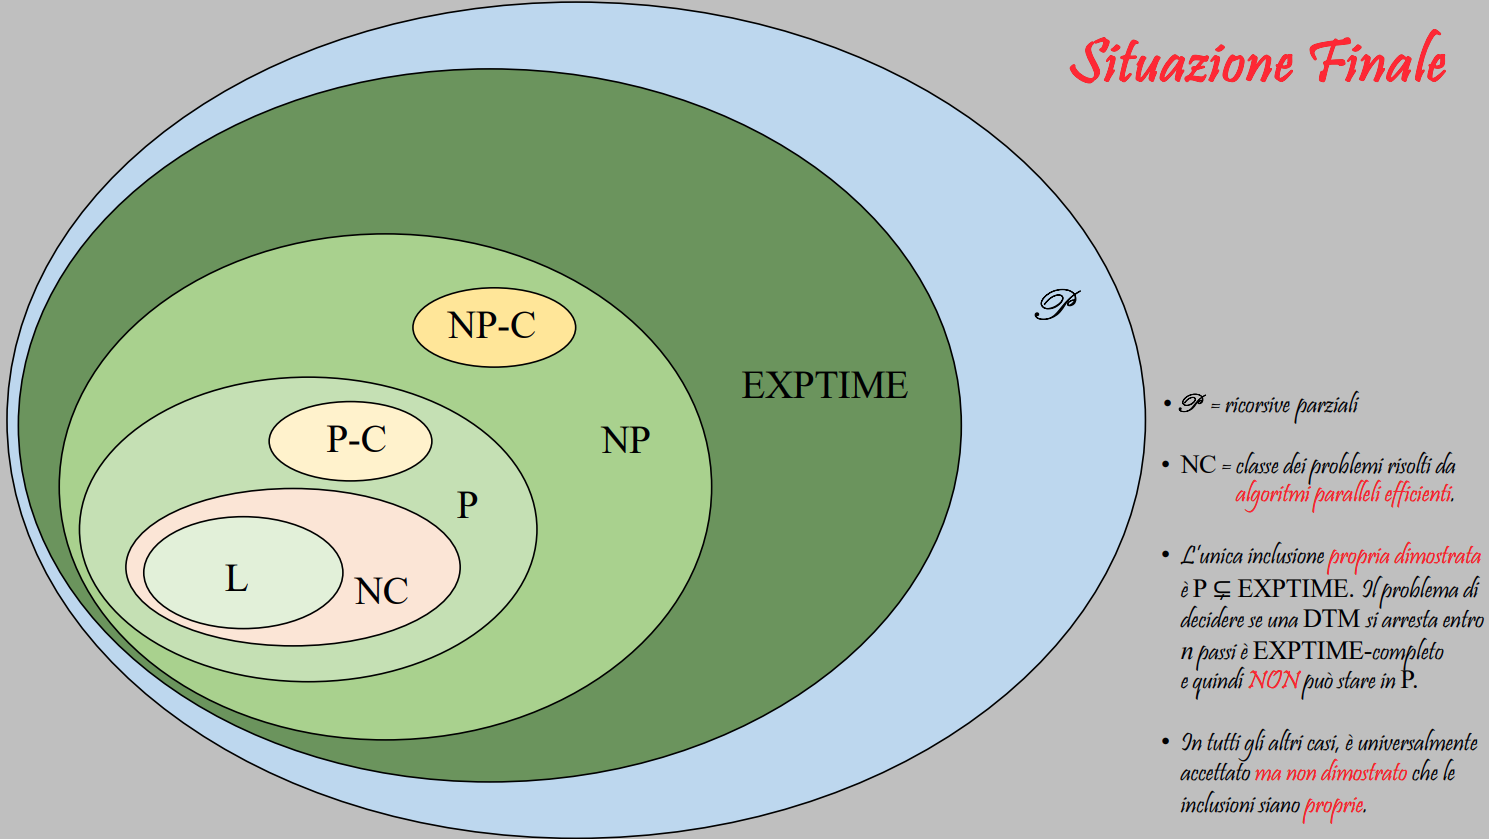
\includegraphics[width=1\textwidth]{img/finale.png}
\end{figure}


%%% Local Variables:
%%% TeX-master: "../it.tex"
%%% End:
